\documentclass[12pt,oneside]{article}
\usepackage[utf8]{inputenc}
\usepackage{microtype}
\usepackage{wrapfig}
\usepackage{xcolor}
  \definecolor{xred}{HTML}{b02428}
\usepackage{hyperref}
  \hypersetup{colorlinks=true,allcolors=xred}
\pagestyle{empty}
\usepackage[left=1.5in, right=1in, top=1.2in, bottom=1.2in]{geometry}
\usepackage{changepage}
\usepackage{graphicx}
\usepackage[absolute]{textpos}\TPGrid{16}{16}
\usepackage{tikz}
\usepackage{everypage}
  \AddEverypageHook{
    \begin{textblock}{0.5}[0,0](0,0)
      \tikz \node[fill=xred,minimum width=0.5\TPHorizModule,minimum height=16\TPVertModule] {};
    \end{textblock}
    \begin{textblock}{16}[1,1](23,16)
      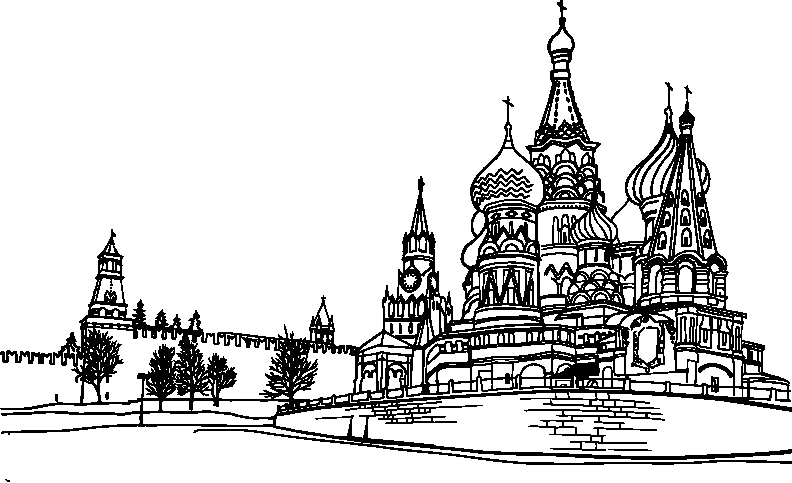
\includegraphics[height=3in]{moscow}
    \end{textblock}
  }
\begin{document}
\fontfamily{cmtt}\selectfont
\raggedbottom
\raggedright
\setlength{\topskip}{6pt}
\setlength{\parindent}{0pt} % indent first line
\setlength{\parskip}{6pt} % before par

\begin{wraptable}{r}{1.2in}%
  \raggedleft%
  \includegraphics[height=1.2in]{../logo}
\end{wraptable}

\textcolor{xred}{\bfseries
{\large The First} \\
{\Large International Conference on\\[3pt]
Code Quality (ICCQ)}}

In
\href{https://conferences.ieee.org/conferences_events/conferences/conferencedetails/51190}{cooperation}
with the IEEE Computer Society.

\vspace{6pt}

Moscow, Russia \\
27-Mar-2021 (one day) \\
\href{https://www.iccq.ru}{www.iccq.ru} / \href{https://easychair.org/cfp/ICCQ20}{EasyChair CFP}\\

\vspace{12pt}

\newcommand\person[2]{
  \begin{minipage}[t]{0.22\textwidth}\raggedright%
  \includegraphics[height=0.6in]{../images/#1} \\
  {\small #2}%
  \end{minipage}
}
\person{keynote/anders-moller}{%
  \href{https://cs.au.dk/~amoeller/}{Anders Møller} \\
  \href{https://www.au.dk/}{Aarhus Uni} \\
  Keynote}%
\person{steering/zhang-yuxin}{%
  \href{https://www.huaweicloud.com/intl/en-us/news/building-a-smart-future-with-full-stack-innovation-for-the-cloud.html}{Zhang Yuxin} \\
  \href{https://www.huaweicloud.com/}{Huawei Cloud} \\
  Steering Chair}%
\person{pc/sergey-zykov}{%
  \href{https://scholar.google.com/citations?user=68uxw-AAAAAJ&hl=en}{Sergey Zykov} \\
  \href{https://www.hse.ru/en/org/persons/3468544}{HSE} \\
  PC Chair}%
\person{orgs/yegor-bugayenko}{%
  \href{https://www.yegor256.com/about-me.html}{Yegor Bugayenko} \\
  \href{https://career.huawei.ru/rri/}{Huawei RRI} \\
  Orgs Chair}

\vspace{6pt}

We believe that the quality of the source code that millions of programmers
write every day could be much higher than it is now. We believe that the
contribution computer science can make to improve this situation is greatly
undervalued. We aim to solve this problem by gathering
together cutting-edge researchers and letting them share their most recent ideas.

Sponsored by and held at \href{https://www.hse.ru/en/}{HSE University}.

% \vspace{6pt}
% Estimated attendance: 150-200 \\
% Estimated number of papers submitted: 50+ \\
% Papers to be accepted: 10

% \vspace{6pt}

Topics: Static Analysis, Bug Detection, Maintainability.

Papers will be published in the \textit{Proceedings of ICCQ},
will appear in IEEE Xplore\textsuperscript{\textregistered},
and will be indexed by Web of Science, Scopus, Google Scholar, DBLP, and others.

Thanks to our partners, publishing will be free.

\vspace{6pt}

Paper submission date: 4 Dec 2020 \\
Author notification: 5 Feb 2021 \\
Camera-ready submissions: 19 Feb 2021

\vspace{6pt}

\begin{adjustwidth}{0pt}{1in}
ICCQ is also sponsored by:
\href{https://www.ispras.ru/en/}{Ivannikov Institute for System Programming (ISP) of the RAS},
\href{https://www.msu.ru/}{Moscow State University (MSU)},
\href{https://mipt.ru/english/}{Moscow Institute of Physics and Technology (MIPT)},
\href{https://russoft.org/en/}{RUSSOFT},
\href{https://2021.secrus.org/?lang=en}{SECR},
\href{https://www.huawei.com}{Huawei},
\href{https://sbercloud.ru/}{SberCloud},
\href{https://yandex.ru/}{Yandex},
\href{https://www.kaspersky.com/}{Kaspersky},
and \href{https://www.iccq.ru/#partners}{others}.
\end{adjustwidth}

\end{document}
